% Template from https://www.overleaf.com/latex/templates/international-university-hcmiu-vnu-pre-thesis-and-thesis-latex-template/hkwcgswxgfth

\documentclass[12pt, twoside]{report}

\usepackage[utf8]{inputenc}
\usepackage{amsmath}
\usepackage{csquotes}
\usepackage{graphicx}
\usepackage[english]{babel}
\usepackage[a4paper, top=1in, bottom=0.8in, left=1in, right=1in]{geometry}
\usepackage{fancyhdr}
\usepackage[colorlinks=true,linkcolor=black]{hyperref}
\usepackage{comment}
\usepackage{float}
\usepackage{tikz}
\usepackage{tikz-qtree}
\usepackage{graphicx}
\usepackage{siunitx}
\usepackage{listings}
\usepackage{algorithm}
\usepackage{algorithmic}

\usetikzlibrary{arrows,automata,positioning}

\lstset{%
	captionpos=b,
	language=Python,
	basicstyle=\ttfamily\footnotesize,
	keywordstyle=\color{blue}\bfseries,
	breaklines=true,
	breakatwhitespace=true,
	frame=single,
	numbers=left,
	numberstyle=\footnotesize,
	numberstyle=\tiny\color{gray},
	stringstyle=\color{orange},
	rulecolor=\color{black},
	title=\lstname,
	showstringspaces=false,
}

\graphicspath{{images/}}

\begin{document}

\pagenumbering{roman}

	\begin{titlepage}

		\renewcommand{\thesection}{\arabic{section}}
		\newcommand{\HRule}{\rule{\linewidth}{0.2mm}}
		
		\center

		\textsc{\Large Ca' Foscari University of Venice }\\[1.0cm]
		
\includegraphics[scale=0.85]{ unive-emblem.png }\\[1cm]
		\textsc{\Large Department of Environmental Sciences, Informatics and Statistics }\\[0.5cm]
		\textsc{\large MCS Computer Science and Information Technology CM-90 }\\[0.5cm]
		\textsc{\large [CM0481] Software Performance and Scalability }\\[0.5cm]
		
		\HRule \\[0.8cm]
		{ \Huge \bfseries IMDb: Performance and Scalability Analysis }\\[0.5cm]
		\HRule \\[0.8cm]
		
		\Large \emph{Authors:}\\
		Michele \textsc{Lotto} - {\normalsize 875922}\\
		Daniel Jader \textsc{Pellattiero} - {\normalsize 903837}\\[3.5cm]

		{\large Rev. 26/06/2024  }\\
		
		\vfill

	\end{titlepage}

\tableofcontents
\listoftables
\addcontentsline{toc}{chapter}{List of Tables}
\listoffigures
\addcontentsline{toc}{chapter}{List of Figures}
\lstlistoflistings
\addcontentsline{toc}{chapter}{List of Listings}

\chapter*{Abstract}
\addcontentsline{toc}{chapter}{Abstract}
This report presents a comprehensive account of the implementation and performance testing process conducted on a web application that emulates the IMDb website\footnote[1]{https://www.imdb.com/}.

The report begins with an overview of the system implementation, in which the technologies utilized are outlined. Subsequently, a theoretical analysis of the queueing system network is presented, in which the implemented system is characterised.
The load test conducted on the system will be subjected to a thorough examination, including an analysis of its theoretical and empirical findings.

In conclusion, a potential architectural solution is evaluated for its potential to enhance the scalability of the tested system.

It should be noted that the implementation of the system, along with all automated programs and scripts referenced in this report, is fully documented and accessible on the GitHub repository\footnote[2]{https://github.com/danieljaderpellattiero/unive-imdb}.


% Body of the paper
\chapter{System implementation}
\pagenumbering{arabic}
\setcounter{page}{1}
% Chapter introduction

The project entails the development of a three-tiered web application, comprising a database, a RESTful API and a website.
The following sections will present an analysis of each of these components, with a focus on the technologies and design choices implemented.

\section{Database -- MongoDB}

MongoDB is a popular NoSQL document-oriented database that is designed to store and manage large volumes of structured and unstructured data.

The database was selected as the optimal choice for managing the IMDb Non-Commercial Datasets\footnote[1]{https://developer.imdb.com/non-commercial-datasets/} due to its adoption of a schemaless data modelling, which enables the management of any non-normalised records or fields within the data.
Furthermore, the usage of JSON format for storing the records allows for enhanced efficiency in interactions with the backend.

\subsection{Data analysis}

Each dataset, comprising a UTF-8-encoded tab-separated values (TSV) file, was subjected to analysis using the Python Pandas library.
The primary steps of the data analysis process were as follows:

\begin{enumerate}
	\item The replacement of missing values (denoted by  \verb|`\N'|) with default values of a type consistent with the column domain to which they belong.
	\item The removal of records that lack some data fields.
	\item The normalisation of fields containing arrays of elements.
	\item The potential replacement of table indexes.
\end{enumerate}

Further modifications were implemented to the tables, however, as these affect the database schema, they will be addressed subsequently.

Once the preliminary phase of preparing the datasets was complete, it was decided that the files should be exported in the JSON format, allowing them to be imported into the database.
Additionally, the files were exported also in the Parquet format, enabling them to be uploaded to the GitHub repository via the GitHub Large File Storage (LFS) facility\footnote[2]{https://git-lfs.com/}. 

\subsection{Collections' schema}

MongoDB represents objects using BSON (Binary JSON) types, which are binary-encoded serialisations of documents that adhere to the JSON format.
As each table in MongoDB is translated into the concept of a document collection, the diagrams of the respective collections imported from the datasets obtained post data analysis are presented below.
Furthermore, supplementary notes on the refactoring of the tables are provided.

\begin{table}[H]
	\caption{`\textit{title.basics}' collection schema}
\begin{center}
	%\def\arraystretch{1.4}
	\begin{tabular}{ cccc }
		%\multicolumn{5}{c}{} \\
		\hline
		Field & BSON type & Index & Index type \\
		\hline
		\_id & String & yes & unique, ascending \\
		titleType & String & no & - \\
		name & String & no & - \\
		nameEng & String & no & - \\
		isAdult & Boolean & no & - \\
		genres & Array[String] & no & - \\
		startYear & 32-bit integer & no & - \\
		endYear & 32-bit integer & no & - \\
		runtime & 32-bit integer & no & - \\
		rating & Double & no & - \\
		votes & 32-bit integer & no & - \\
		\hline
	\end{tabular}
\end{center}
\end{table}  

\textit{N.d.R.}: A collection was created ad hoc for records with the field \textit{`titleType'} equal to \textit{`tvEpisode'}.

\begin{table}[H]
	\caption{`\textit{title.akas}' collection schema}
\begin{center}
	%\def\arraystretch{1.4}
	\begin{tabular}{ cccc }
		%\multicolumn{5}{c}{} \\
		\hline
		Field & BSON type & Index & Index type \\
		\hline
		\_id & ObjectId & yes & unique, ascending \\
		titleId & String & no & - \\
		ordering & 32-bit integer & no & - \\
		region & String & no & - \\
		name & String & no & - \\
		nameLower & String & yes & ascending \\
		\hline
	\end{tabular}
\end{center}
\end{table}

\textit{N.d.R.}: \textit{`language'}, \textit{`types'}, \textit{`attributes'}, \textit{`isOriginalTitle'} fields dropped.

\begin{table}[H]
	\caption{`\textit{title.crew}' collection schema}
\begin{center}
	%\def\arraystretch{1.4}
	\begin{tabular}{ cccc }
		%\multicolumn{5}{c}{} \\
		\hline
		Field & BSON type & Index & Index type \\
		\hline
		\_id & String & yes & unique, ascending \\
		writers & Array[String] & no & - \\
		directors & Array[String] & no & - \\
		\hline
	\end{tabular}
\end{center}
\end{table}

\begin{table}[H]
	\caption{`\textit{title.episodes}' collection schema}
\begin{center}
	%\def\arraystretch{1.4}
	\begin{tabular}{ cccc }
		%\multicolumn{5}{c}{} \\
		\hline
		Field & BSON type & Index & Index type \\
		\hline
		\_id & String & yes & unique, ascending \\
		titleId & String & yes & ascending \\
		name & String & no & - \\
		nameEng & String & no & - \\
		season & 32-bit integer & no & - \\
		episode & 32-bit integer & no & - \\
		isAdult & Boolean & no & - \\
		genres & Array[String] & no & - \\
		startYear & 32-bit integer & no & - \\
		endYear & 32-bit integer & no & - \\
		runtime & 32-bit integer & no & - \\
		rating & Double & no & - \\
		votes & 32-bit integer & no & - \\
		\hline
	\end{tabular}
\end{center}
\end{table}

\begin{table}[H]
	\caption{`\textit{name.basics}' collection schema}
	\begin{center}
		%\def\arraystretch{1.4}
		\begin{tabular}{ cccc }
			%\multicolumn{5}{c}{} \\
			\hline
			Field & BSON type & Index & Index type \\
			\hline
			\_id & String & yes & unique, ascending \\
			fullName & String & no & - \\
			birth & 32-bit integer & no & - \\
			death & 32-bit integer & no & - \\
			professions & Array[String] & no & - \\
			\hline
		\end{tabular}
	\end{center}
\end{table}

\textit{N.d.R.}: \textit{`knownForTitles'} field dropped.

\begin{table}[H]
	\caption{`\textit{title.principals}' collection schema}
\begin{center}
	%\def\arraystretch{1.4}
	\begin{tabular}{ cccc }
		%\multicolumn{5}{c}{} \\
		\hline
		Field & BSON type & Index & Index type \\
		\hline
		\_id & ObjectId & yes & unique, ascending \\
		titleId & String & yes & ascending \\
		ordering & 32-bit integer & no & - \\
		personId & String & no & - \\
		job & String & no & - \\
		characters & Array[String] & no & - \\
		\hline
	\end{tabular}
\end{center}
\end{table}

\textit{N.d.R.}: \textit{`category'} field used to fill empty \textit{`job'} fields; then dropped.

\subsection{Schema indexes and bulk data insert}

As can be seen from the tables above, in addition to the standard unique indexes, it was decided to add additional ones to optimise the queries requested by the backend.
Given the significant use of wildcard searches based on regular prefix expressions, it was decided to implement ascending indexes on several \textit{`String'} type fields to drastically reduce search times without having to resort to a text index, which would take up much more space due to the tokenisation and stemming of the fields.

In order to perform a bulk insert of the approximately 42.5 million records contained in $\sim1.6$ GB of JSON files, it was decided to write a script in Python that would take advantage of a multithreaded execution of the \verb|mongoimport| command-line tool provided by MongoDB.
The overall script is responsible for generating the database's collections, populating them and finally creating indexes.

\subsection{Technical details}

The database was configured as a locally managed instance of MongoDB, thus avoiding the utilisation of the cloud version of the service (Atlas).
The service's local deployment facilitated the monitoring and control of its resources, as well as the measurement of its performance.
These factors collectively contributed to the generation of more reliable results during the load tests that were conducted.

Technical insights into the environment are presented below.

\begin{itemize}
	\item MongoDB 7.0.11 (Community Server service)
	\item MongoDB Compass 1.43.3 (database UI)
	\item MongoDB Shell 2.2.9 (database CLI)
\end{itemize}

\section{RESTful API -- Express}

The web application's backend was developed using the Express framework, a Node.js web application framework that was identified as the most widely utilised in the `State of JavaScript 2023' survey\footnote[3]{https://2023.stateofjs.com/en-US/other-tools/\#backend\_frameworks}.

A variety of endpoints were incorporated into the API, enabling a constrained yet still functional utilisation of the web interface.
The user-accessible API calls are enumerated below, along with a concise description of each.

\begin{enumerate}
	\item \verb|localhost:3000/search/preview/:title| -- Returns the top 4 most voted titles that match the search query prefix.
	\item \verb|localhost:3000/search/:title| -- Returns the most voted titles that match the search query prefix; the results are paginated in groups of 8.
	\item \verb|localhost:3000/search/episodes/:title| -- Returns the episodes of a specific title that matches the \textit{`titleId'} parameter.
	\item \verb|localhost:3000/title/:id| -- Returns the details of a specific title that matches the \textit{`\_id'} parameter.
	\item \verb|localhost:3000/episode/:id| -- Returns the details of a specific episode that matches the \textit{`\_id'} parameter.
\end{enumerate}

The official MongoDB driver for Node.js (Typescript) \verb|mongodb@6.8| is responsible for handling queries from the backend to the database.
We deliberately decided not to utilise any form of Object-Relational/Document Mapping (e.g. \verb|Mongoose| or \verb|Prisma|) due to the suitability of the JSON record format to the application domain model and potential performance overheads.

Aggregation pipelines are used to facilitate the execution of queries to the database.
These pipelines allow the definition of queries through the use of a sequential list of stages, thereby simplifying the grouping and sorting of data and providing control over the execution times of the individual stages within the pipeline.

\section{Website -- Vue and Tailwind CSS}

The web interface of the system was realised using Vue.js `The Progressive JavaScript Framework', a well-known framework used for building SPAs (Single Page Applications) renowned for its component-based architecture and reactive data binding system.
The aesthetic component was addressed through the utilisation of Tailwind CSS, a utility-first CSS framework that can be suitably integrated with Vue.
A bundle of the website, optimised for deployment on a static hosting service, was created at the end of the development process using Vite\footnote[4]{A modern front-end build tool that facilitates optimized production builds through the utilization of ES hot module replacement (HMR).}.
This design choice ensures that the frontend is efficiently packaged into static files, which can be served directly to users without requiring server-side processing.
Consequently, during load testing with JMeter, the focus has been exclusively on the backend API endpoints, as the frontend's static nature does not impose additional load on the server.

Thumbnails of the web interface are available on GitHub\footnote[5]{https://github.com/danieljaderpellattiero/unive-imdb/tree/frontend/thumbnails}.


\chapter{Test case identification}
\section{High-level test case design}

This brief chapter aims to present the test case designed to perform the load test of the system.
In order to illustrate the user behaviour modelled by the test, we define a trivial finite-state automata with reference to the endpoints implemented in the RESTful API.

It should be noted that, although this aspect will be discussed in greater detail in the following chapters, the two endpoints that will be used in the load test result in two different classes of jobs, which must consequently be analysed individually.

\begin{center}
	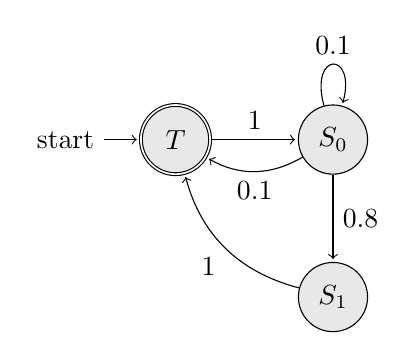
\begin{tikzpicture}[shorten >=1pt,node distance=2cm,on grid,auto]
		\tikzstyle{every state}=[fill={rgb:black,1;white,10}]
		\node[state, initial, accepting] (0) {$T$};
		\node[state] (1) [right of = 0] {$S_0$};
		\node[state] (2) [below of = 1] {$S_1$};
		\path[->]
		(0) edge node {1} (1)
		(1) edge [loop above] node {0.1} (1)
		(1) edge [bend left] node {0.1} (0)
		(1) edge node {0.8} (2)
		(2) edge [bend left] node {1} (0);
		;
	\end{tikzpicture}
\end{center}

The above automata has to be interpreted in the following manner:

\begin{itemize}
	\item The user initiates a title search by name match, regardless of the customer language locale. (\verb|/search/:title| -- node $S_{0}$)
	\begin{itemize}
		\item In $80\%$ of cases, the search continues with a precise request for the title information. (\verb|/title/:id| \textit{or} \verb|/episode/:id| -- node $S_{1}$)
		\item In $20\%$ of cases, either the user terminates the search process pre-emptively, without finding the title, thus entering a thinking state -- (node $T$) or it continues the search by hitting the same endpoint though the use of pagination. (\verb|/search/:title?page=n| -- node $S_{0}$)
	\end{itemize}
	\item Upon receipt of the searched title information, the user is satisfied and returns to a thinking state before repeating a new search.
\end{itemize}

\clearpage

\section{Computational settings}

The following table provides an overview of the hardware specifications of the computers utilized in the load test.

\begin{table}[H]
	\caption{Hardware specifications}
\begin{center}
	%\def\arraystretch{1.4}
	\begin{tabular}{ ccccc }
		%\multicolumn{5}{c}{} \\
		\hline
		Machine type & Role & O.S. & CPU & RAM \\
		\hline
		Desktop & Benchmark executor & Ubuntu 22.04 & Intel i5-13600K (20) & 64 GB \\
		Laptop & System under test & Ubuntu 22.04 & Intel i5-8265U (8) & 8 GB \\
		\hline
	\end{tabular}
\end{center}
\end{table}


\chapter{Queueing network model}
\section{Introduction}

This chapter presents a comprehensive theoretical analysis of the implemented model.
The following illustration depicts the system components involved in the load test in the context of queuing theory. 

For the purposes of this illustration, let Q\textsubscript{T} represent the thinking station, Q\textsubscript{B} represent the backend, and Q\textsubscript{D} represent the database.
It is important to note that within the labels associated with the arcs, the first number indicates the class of the job leaving the station, while the second number indicates the class of the job at the destination station. 

\begin{center}
	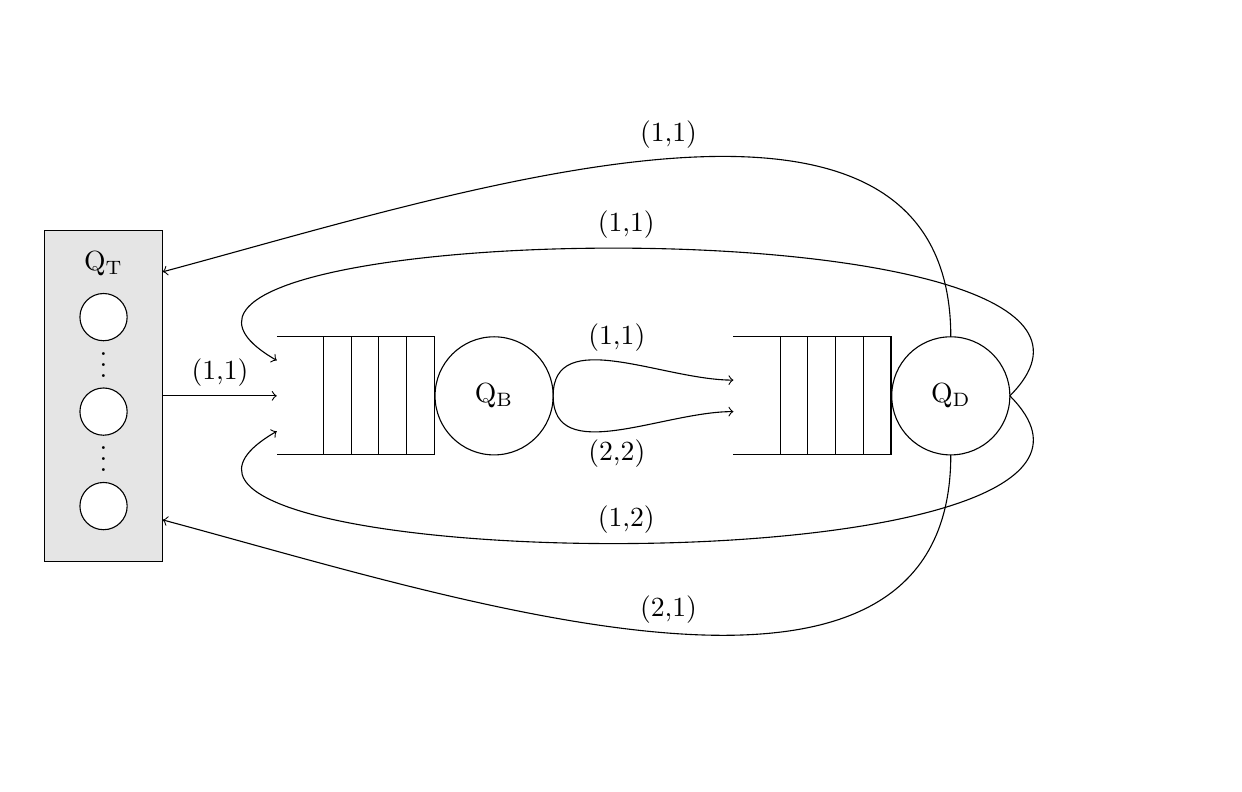
\begin{tikzpicture}[scale=1.0, transform shape]
		\tikzstyle{thinking_station} = [rectangle, draw, minimum height=4.2cm, minimum width=1.5cm, fill=gray!20, align=left]
		\tikzstyle{circle_node} = [circle, draw, fill=white, minimum size=6mm, inner sep=0pt]
		\tikzstyle{queue} = [circle, draw, minimum size=1cm, text centered, inner sep=0pt]
	
		% Thinking station
		\node (QT) [thinking_station] at (0,0) {};
		\node at (0,1.68) {Q\textsubscript{T}};
		% Users belonging to the closed loop
		\node[circle_node] at (0, 1) {};
		\node at (0, 0.5) {$\vdots$};
		\node[circle_node] at (0, -0.2) {};
		\node at (0, -0.7) {$\vdots$};
		\node[circle_node] at (0, -1.4) {};
	
		% Backend station
		% Queue
		\draw (2.2,0.75) -- ++(2cm,0) -- ++(0,-1.5cm) -- ++(-2cm,0);
		\foreach \i in {1,...,4}
		\draw (4.2cm-\i*10pt,0.75) -- +(0,-1.5cm);
		% Service room
		\draw (4.96,-0.00cm) circle [radius=0.75cm];
		% Label service time
		\node at (4.96,-0.00cm) {Q\textsubscript{B}};
	
		% Database station
		% Queue
		\draw (8.0,0.75) -- ++(2cm,0) -- ++(0,-1.5cm) -- ++(-2cm,0);
		\foreach \i in {1,...,4}
		\draw (10cm-\i*10pt,0.75) -- +(0,-1.5cm);
		% Service room
		\draw (10.760,-0.00cm) circle [radius=0.75cm];
		% Label service time
		\node at (10.760,-0.00cm) {Q\textsubscript{D}};
	
		\draw[->]	(QT) to[out=0,in=180] node[above]	{(1,1)} (2.2,0);
		\draw[->]	(5.71,0) to[out=90,in=180] node[above]	{(1,1)} (8.0,0.20);
		\draw[->]	(5.71,0) to[out=-90,in=180] node[below]	{(2,2)} (8.0,-0.20);
		\draw[->]	(11.51,0) to[out=45,in=150] node[above]	{(1,1)} (2.2,0.45);
		\draw[->]	(11.51,0) to[out=-45,in=-150] node[above]	{(1,2)} (2.2,-0.45);
		\draw[->]	(10.760,-0.75) to[out=-90,in=-15] node[above]	{(2,1)} (0.75,-1.575);
		\draw[->]	(10.760,0.75) to[out=90,in=15] node[above]	{(1,1)} (0.75,1.575);
	\end{tikzpicture}
\end{center}

It is possible to derive several characteristics of the system under consideration from the illustration above.

The system is characterised by a closed and interactive nature, free of stability conditions, and a constant number of users that dictate the nature of the workload.
A further aspect that emerges relates to the multiclass nature of the jobs within the system, as indicated by the labels placed at the station entry and exit arcs.

Subsequently, an in-depth examination will be conducted on the distinct service time/demand and probabilistic routing for the two classes of jobs.

In conclusion, the network under analysis can be classified as a BCMP, exhibiting a closed topology and utilising ``Processor Sharing'' (PS) as its scheduling discipline.

Prior to examining the nature of the queues that characterise our network and their associated scheduling disciplines, we proceed with the formalisation and resolution of the network's traffic equations.
These equations will then be essential in producing the theoretical analysis of the system.

\section{Traffic equations}

The system's traffic equations are presented below.

\[
	\begin{array}{c}
	\begin{bmatrix}
	p_{T1B1} \\
	p_{B1D1} \\
	p_{B2D2} \\
	p_{D1B1} \\
	p_{D1B2} \\
	p_{D1T1} \\
	p_{D2T1}
	\end{bmatrix}
	=
	\begin{pmatrix}
	1.0 \\
	1.0 \\
	1.0 \\
	0.1 \\
	0.8 \\
	0.1 \\
	1.0
	\end{pmatrix}
	\end{array}
	\quad : \quad
	\begin{cases}
	\begin{aligned}
	e_{B1} &= e_{T1} + (p_{D1B1} \times e_{D1}) \\
	e_{B2} &= p_{D1B2} \times e_{D1} \\
	e_{D1} &= e_{B1} \\
	e_{D2} &= e_{B2} \\
	e_{T1} &= e_{D2} + (p_{D1T1} \times e_{D1}) \\
	\end{aligned}
	\end{cases}
	\Rightarrow
	\begin{cases}
	\begin{aligned}
	% Insert your new system here, for example:
	e_{B1} &= \num[round-mode=places, round-precision=4]{1.11111111111111} \times e_{T1}  \\
	e_{B2} &= \num[round-mode=places, round-precision=4]{0.888888888888889} \times e_{T1}  \\
	e_{D1} &= \num[round-mode=places, round-precision=4]{1.11111111111111} \times e_{T1}  \\
	e_{D2} &= \num[round-mode=places, round-precision=4]{0.888888888888889} \times e_{T1}  \\
	\end{aligned}
	\end{cases}
\]

The system of equations above demonstrates that our routing is irreducible, which implies that any queue can be accessed from any other queue within the network.
From an analytical standpoint, our system is under-determined, indicating the existence of an infinite number of solutions. The non-trivial solutions can be derived from the non-zero multiplicative coefficients.

Moreover, it is essential to highlight that within this context, where the system under consideration is an interactive queueing network, it is imperative to impose an additional constraint on the previous system, specifically $e_{T1}=1$, given that this is the thinking station Q\textsubscript{T}.

\section{Queueing network components}

This section will provide a brief overview of the components of our network, with reference to Kendall's notation.

\subsection{Thinking station}

The thinking station can be represented by a queuing system described with the \newline ``G/D/$\infty$/IS'' notation.
The distribution of inter-arrival times for jobs at the thinking station is unknown, but the distribution of service times is known, as the jobs within it remain in service (\textit{thinking state}) for a fixed constant time, known as thinking time.
By definition, the thinking station is equipped with an infinite number of servers, indeed an undefined number of jobs can access it.
Consequently, the service discipline of this system is of the ``Delay center'' or ``Infinite Servers'' type, as all the jobs remain in an idle state in parallel.

\subsection{Backend station}

With regard to the JavaScript runtime environment Node.js, despite its reputation as a ``purely single-threaded'' execution environment due to its Event Loop, it is in fact capable of offloading I/O blocking operations to separate threads or the operating system, thus allowing the main thread to continue processing other tasks.
The library that permits the dispatching of blocking operations to a thread pool is called \verb|libuv| and it belongs to the Chrome V8 Engine.
Furthermore, Node.js has also implemented the \verb|worker_threads| module, which allows for further enhancements of performance by the utilisation of multi-core processors for CPU-bound operations.

In light of the aforementioned considerations, it can be concluded that the RESTful API functions as a ``G/G/1/PS'' queueing system.
This is due to the fact that no manual instantiation of multiple worker threads was performed for the API, and thus a unique main thread is responsible for handling all incoming requests through a ``Processor Sharing'' scheduling discipline.

\subsection{Database station}

With regard to MongoDB, an examination of the ``Production Notes'' section reveals that its WiredTiger storage engine is inherently multithreaded.
In particular, the total number of active threads (i.e. concurrent operations) relative to the number of available CPUs can impact performance as follows:

\begin{itemize}
	\item The throughput increases in direct proportion to the number of concurrent active operations, up to the overall number of CPUs.
	\item The throughput decreases as the number of concurrent active operations exceeds the number of CPUs by a certain threshold amount.
\end{itemize}

The optimal number of concurrent active operations for a given application can be determined through the measurement of throughput.

In order to ascertain the exactness of the information provided in the documentation, an empirical test was conducted to monitor the thread pool instantiated by the MongoDB service in both idle and stressed states.

The results obtained from the Linux command-line utility \verb|htop| are presented below.

\begin{figure}[h]
    \centering
    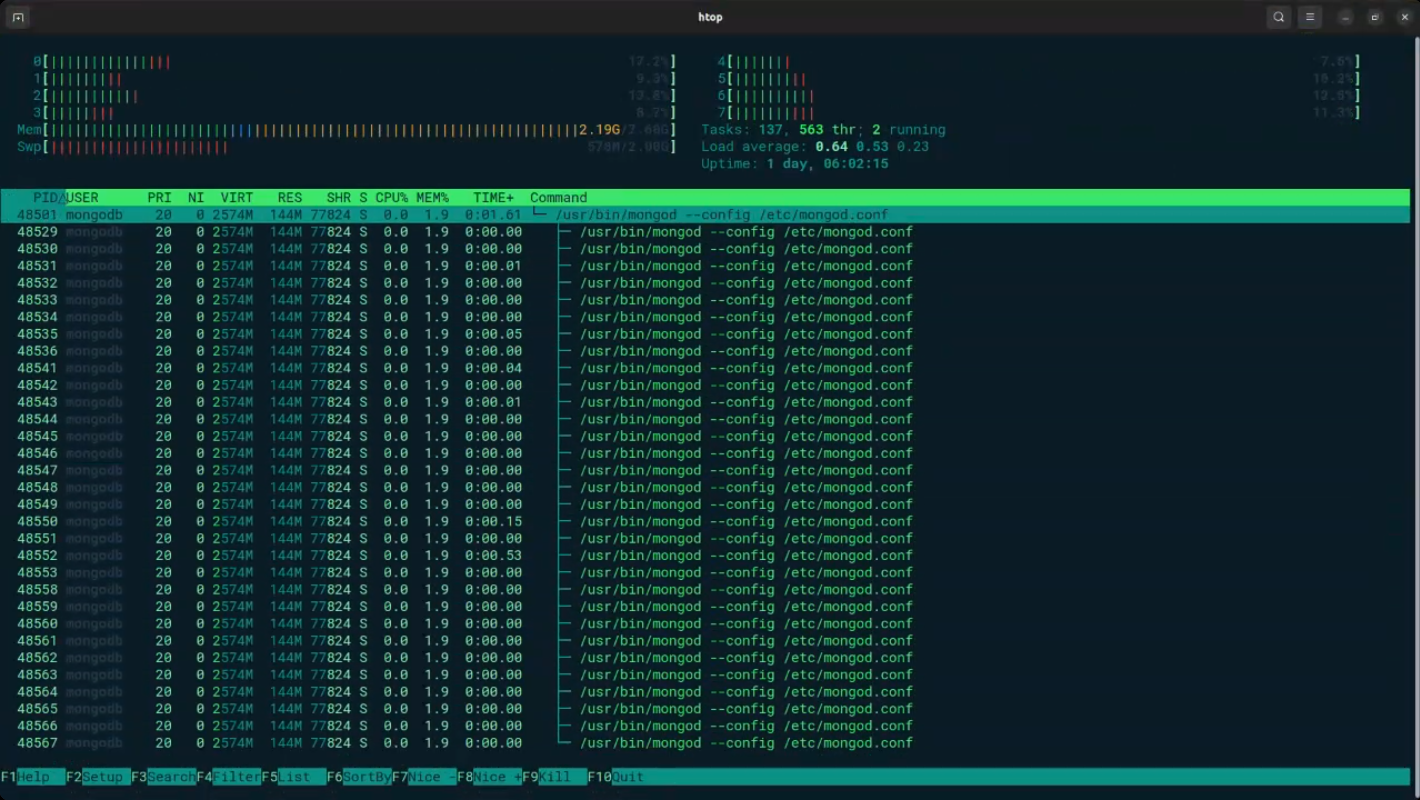
\includegraphics[width=\linewidth]{003/mongo-idle.png}
    \caption{MongoDB thread pool in idle state}
\end{figure}

\begin{figure}[h]
	\centering
	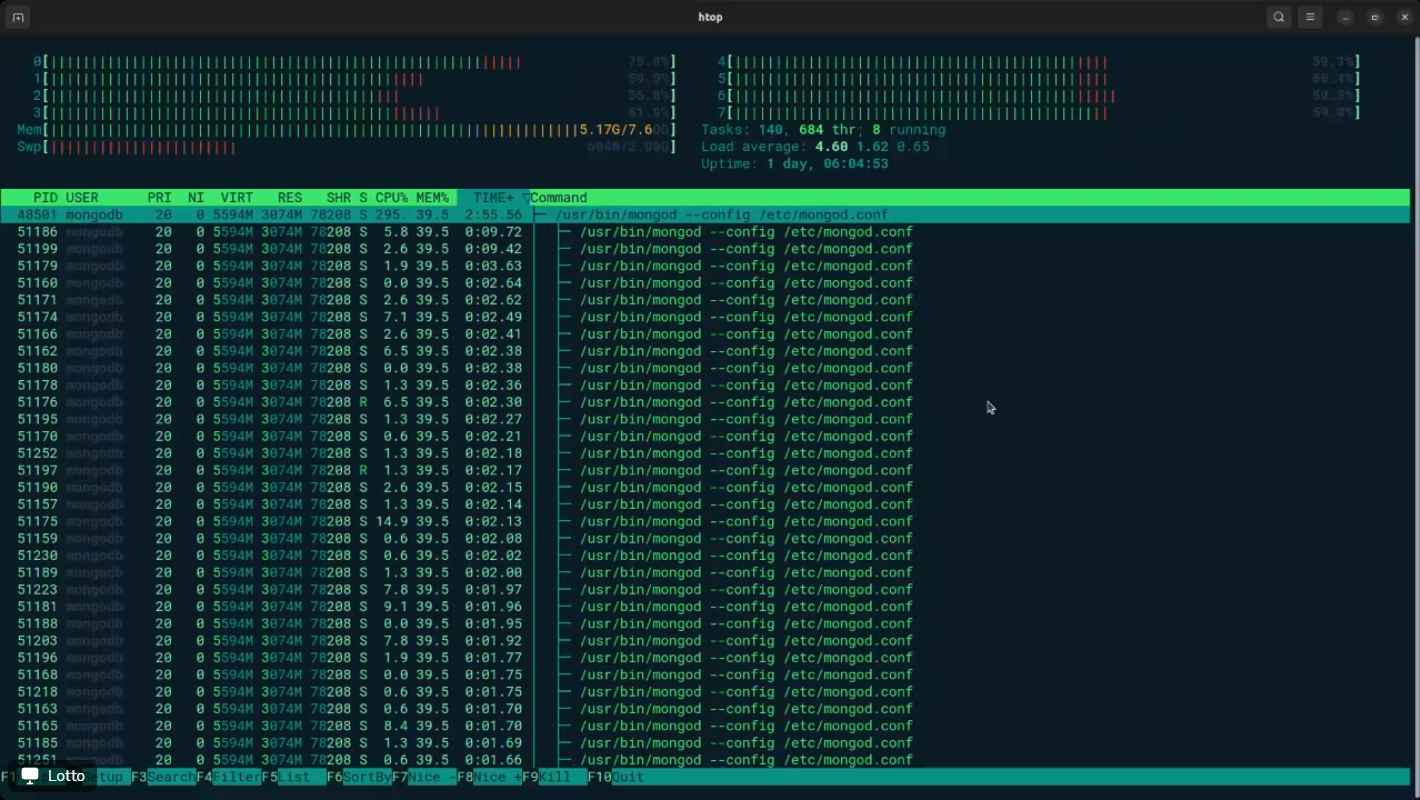
\includegraphics[width=\linewidth]{003/mongo-stress.png}
	\caption{MongoDB thread pool under load conditions}
\end{figure}	

In conclusion, the database can be identified as a ``G/G/\#C/PS'' queueing system, where ``\#C'' represents the number of cores.
The inter-arrival times and service times are both unknown, however it can be stated that the database leverages all CPU cores with a ``Processor Sharing'' service discipline.


\chapter{Q.N. Theoretical analysis}
To fulfil the requirements of the assignment, it is necessary to undertake a comprehensive theoretical analysis of the queueing network.

In order to apply the theoretical notions learned during the course to the estimation of the degree of scalability of the system, the optimal number of users and the identification of the bottleneck of the system, it is first necessary to measure the service times for the queueing network components with regard to the two classes of jobs previously defined.

Although the queries to the endpoint \verb|`/search/:title?page=n'| may vary depending on the parameterization of the URL, we assume that they belong to the same job class.
This assumption will be subsequently confirmed by the empirical results.

\section{Service times measurements}

\subsection{Overview}

Given that we are operating in a ``Processor Sharing'' regime, it is possible for us to exploit the fact that, in the event that there is only one job within the system, its service time is in fact equivalent to the response time.
In light of these considerations, we employed JMeter, a load testing software that will be discussed in greater detail later on, to perform two tests (one for each class of jobs) with the objective of measuring the various service times of our stations.

Both tests comprise a user (a thread) executing a request to the RESTful API at a constant interval of 1 second.
In both cases, the user makes a total of 100 queries, a number determined by the size of the query set imposed by the task, which allows a good normal approximation.

Details on the tests carried out are provided in the following sections.

\subsection{Test query set}

A Python script was employed to perform a random sampling with reinsertion of 10,000 movie titles based on our MongoDB collections.

It was assumed that the probability of a movie being selected in the extraction is proportional to the number of votes it received.
In order to obtain the most comprehensive query set possible, it was decided to include all movies, all episodes, and all the various linguistic declinations of these in the extraction.
The entire process was carried out using the \verb|pandas.DataFrame.sample| function.

\subsection{RESTful API Profiling}

To obtain the most precise measurement of service times for the two classes of jobs, two different versions of the backend were implemented.
One was employed for load testing and the other was used for the current employment; the latter version contained mechanisms to perform profiling on its execution.

Indeed, within the API, it was necessary to distinguish between the processing times of code in Node.js and those of database aggregation pipelines.
To perform profiling on the Express execution, it was decided to utilise the \verb|PerformanceObserver| Node interface, which forms part of the Performance Timing API.
Indeed, this interface enabled the effective measurement of execution times without the addition of overheads through the utilisation of the \verb|Marks|, namely high-resolution timestamps.

Conversely, regarding MongoDB profiling, the situation was more intricate.
In order to facilitate the process, we proceeded to activate the \verb|system.profile| collection within our database. 
This is a \textit{capped collection}\footnote[1]{A fixed-size collection that performs document insertion and retrieval based on the order in which they were added, exhibiting behaviour analogous to that of circular buffers.} that is created by default by the MongoDB Profiler for each database and hidden from the user.
Its purpose is to measure precise metrics regarding CRUD operations and other administrative and/or configuration commands executed on a running instance of MongoDB.
Consequently, the utilisation of the profiler enabled the accurate determination of the execution times inherent to the aggregation pipelines.

Upon completion of the whole process, all metrics evaluated by the API execution are transcribed asynchronously, thus maintaining optimal performance, by \verb|Pino|.

\verb|Pino.js| is a fast and lightweight Node.js logging library: it is a robust and scalable solution due to its comprehensive asynchronous logging of JSON-formatted files that provides customizable log levels and serializers while maintaining low processing costs.

\subsection{Empirical service times}

Following the execution of the two tests with JMeter, the service times of our system components with respect to the job classes identified in our network are as follows:

\[
\mu^{-1}_{B1} = \num[round-mode=places, round-precision=5]{0.0016899999999999999} \, \text{s}
\quad \quad
\mu^{-1}_{D1} = \num[round-mode=places, round-precision=5]{0.00257625} \, \text{s}
\quad \quad
\mu^{-1}_{B2} = \num[round-mode=places, round-precision=5]{0.00171} \, \text{s}
\quad \quad
\mu^{-1}_{D2} = \num[round-mode=places, round-precision=5]{0.0014637500000000002} \, \text{s}
\]

It should be noted that, although MongoDB employs a scheduling discipline of the ``Processor Sharing'' type, it is not a single-server system analogous to the M/G/1/PS queues analysed during the course.
However, since we must assume that we are dealing with a single server station, in order to be able to compute, for instance, the asymptotic bounds for the throughput and the expected response time (part of the theoretical analysis carried out in the following chapters), it is necessary to treat the database as if it were a single server, and therefore to calculate its service time in the following way:
\[
	\mu^{-1}_{Dx} = \frac{\overline{R}}{\text{number of CPUs}} \quad \text{where} \quad x \in \{1, 2\}
\]

\section{Bottleneck identification}

Thus far, we have calculated the service times of each station per job class and the relative visit ratios ($\overline{V}_{i}$).
These $\overline{V}_{i}$ are derived from the solutions of the traffic equations and indicate the expected number of visits to each station with respect to each visit made to the reference station (Q\textsubscript{T}).

\[
\overline{V}_{B1} = \num[round-mode=places, round-precision=5]{1.11111111111111}
\quad
\overline{V}_{D1} = \num[round-mode=places, round-precision=5]{1.11111111111111}
\quad
\overline{V}_{B2} = \num[round-mode=places, round-precision=5]{0.888888888888889}
\quad
\overline{V}_{D2} = \num[round-mode=places, round-precision=5]{0.888888888888889}
\quad
\overline{V}_{T} = \num[round-mode=places, round-precision=5]{1.00000000000000}
\]

The data enables the calculation of the service demands ($\overline{D}_i$), which represent the quantity of service requested by a user from each station for each visit to the reference station.
This is achieved through the application of the following formula:

\label{eq:service-demands}
\begin{equation}
	\overline{D}_i = \overline{V}_i \times \mu^{-1}_i \quad \text{where} \quad i \in \{B1, D1, B2, D2\}
\end{equation}

\[
\overline{D}_{B1} = \num[round-mode=places, round-precision=5]{0.00187777777777778}
\quad
\overline{D}_{D1} = \num[round-mode=places, round-precision=5]{0.00286250000000000}
\quad
\overline{D}_{B2} = \num[round-mode=places, round-precision=5]{0.00152000000000000}
\quad
\overline{D}_{D2} = \num[round-mode=places, round-precision=5]{0.00130111111111111}
\]

The results indicate that the database is the bottleneck station. 
A further calculation of the utilisation of each station can be made using the Bottleneck Law:

\label{eq:bottleneck-law}
\begin{equation}
	\rho_i = X_1 \times \overline{D}_i \quad \text{where} \quad i \in \{B1, D1, B2, D2\}
\end{equation}

A graph is provided below, which illustrates the varying levels of station utilisation over the number of users.

\begin{figure}[h]
	\centering
	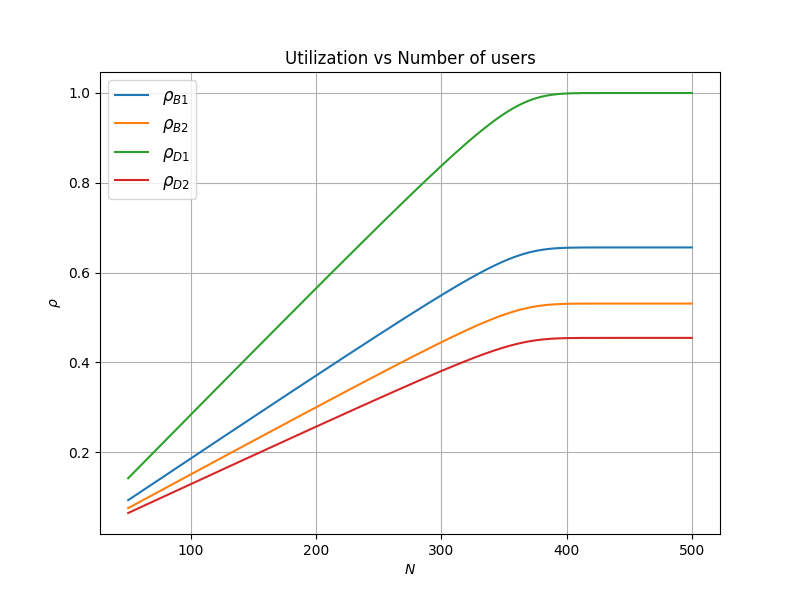
\includegraphics[width=\linewidth]{004/stations-utilization.png}
	\caption{Stations utilisation over the number of users}
\end{figure}

It can be concluded that the database is the component with the highest utilisation rate.

\section{Asymptotic bounds}

In the next section, we will perform a mean value analysis to compute the expected performance indices of our system.
This will be done through Little's Law and the recursive procedure on which this technique is based, without the need to compute the normalization constant G\textsubscript{K} required by Gordon Newell's Theorem.

Prior to conducting the previously announced analysis, a preliminary calculation is conducted using a Python script to determine the upper and lower bounds of response time ($\overline{R}$) and throughput ($X$) in relation to the number of customers in the network.

This is done according to the following formulas:

\label{eq:asymptotic-bounds-expected-response-time}
\begin{equation}
	\overline{R} \geq max\left(\overline{D},N\overline{D}_b-\overline{Z}\right)
\end{equation}

\label{eq:asymptotic-bounds-throughput}
\begin{equation}
	X \leq min\left(\frac{N}{\overline{D}+\overline{Z}},\,\frac{1}{\overline{D}_b}\right) \quad \text{where}
\end{equation}
\[
	\quad \overline{Z} \quad \text{exp. thinking time,} \quad \overline{D}_b \quad \text{bottleneck service demand,} \quad \overline{D} = \sum^{K}_{j=2}\overline{D}_{j}  \\
\]

The parametric values of the calculated limits are provided below:

\[
 R \geq max\left(\num[round-mode=places, round-precision=5]{0.00756138888888889},\;N\times\num[round-mode=places, round-precision=5]{0.00286250000000000}-1\right) \\
\]

\[
 X \leq min\left(\frac{N}{\num[round-mode=places, round-precision=5]{0.00756138888888889}+1},\;\frac{1}{\num[round-mode=places, round-precision=5]{0.00286250000000000}}\right) \\
\]

\section{Mean Value Analysis}

\subsection{JMVA emulation setup}

In order to estimate the performance indices of our queueing network, we employed the ``Java Modelling Tools (JMT)'' suite of applications developed by the ``Politecnico di Milano''.
In particular, we utilised the JMVA (``Mean Value Analysis and Approximate solution algorithms for queueing network models'') application.

The subsequent steps are those required to prepare the emulation within the software according to our queueing network configuration.

\clearpage

1.
The number of customers (50) and the number of classes of jobs were entered.
As can be seen, only one class was indicated, as only class 1 jobs were output from the thinking station.
\begin{figure}[h]
	\centering
	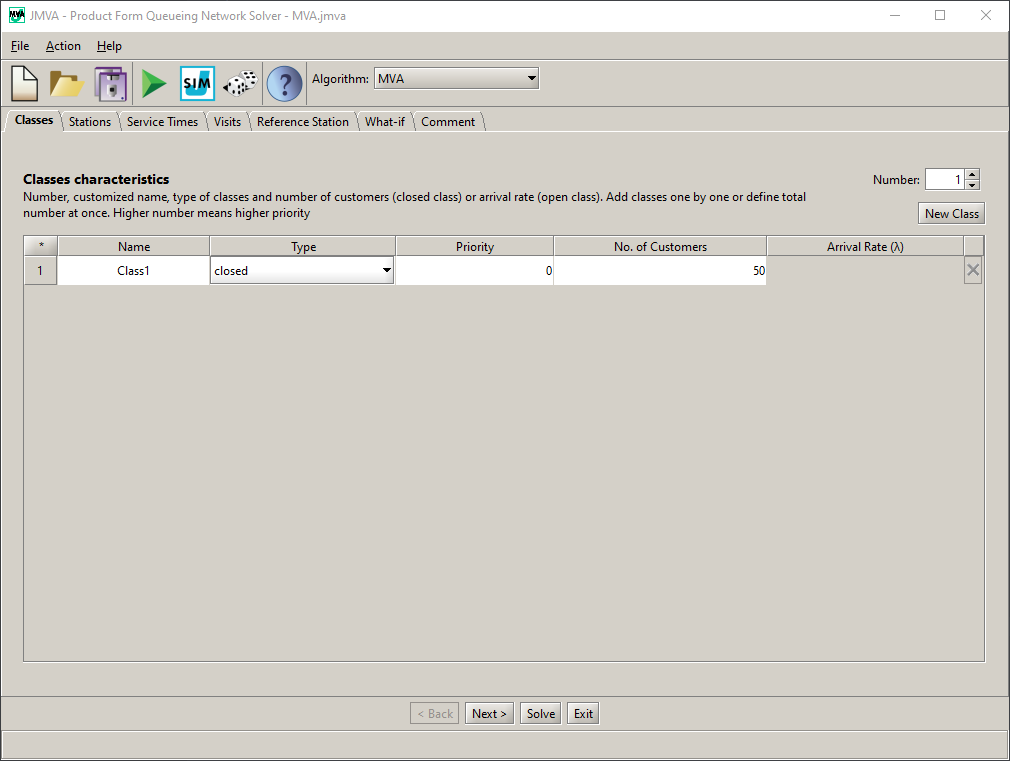
\includegraphics[scale=0.40]{004/JMVA/classes.png}
	\caption{JMVA setup -- classes of jobs}
\end{figure}

2.
The stations in the queueing network are entered according to their respective load type.
The thinking station is designated as a ``delay type'', whereas other stations are classified as ``load-independent'', as their service time remains consistent regardless of the number of customers.
\begin{figure}[h]
	\centering
	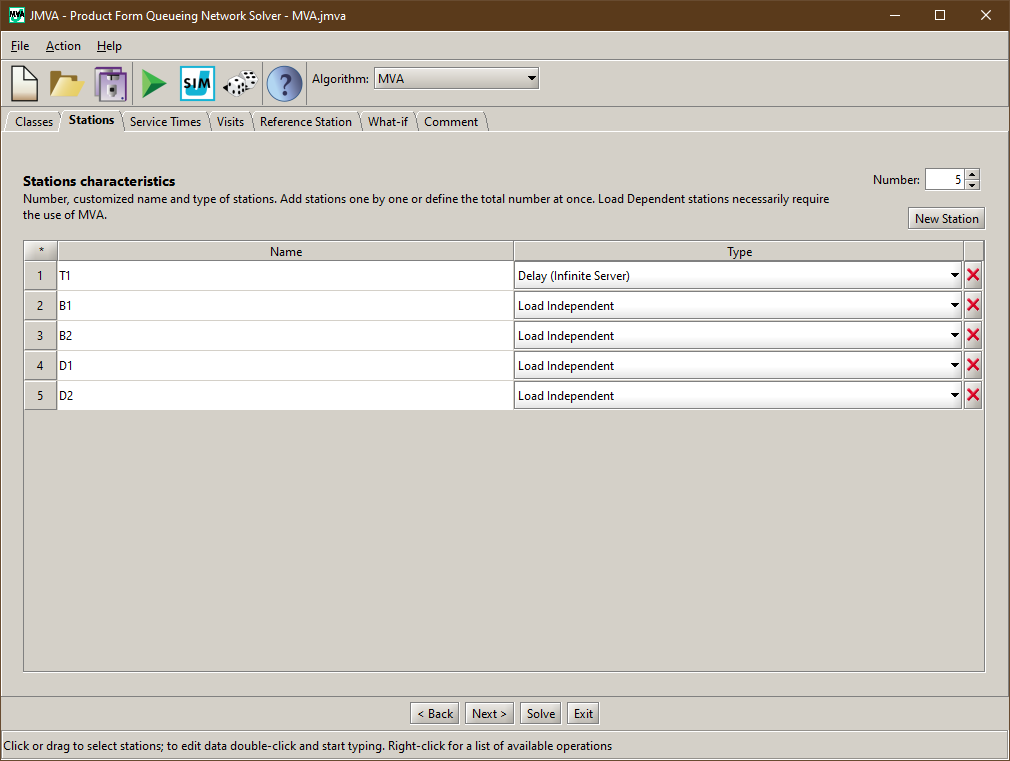
\includegraphics[scale=0.40]{004/JMVA/stations.png}
	\caption{JMVA setup -- stations}
\end{figure}

\clearpage

3.
The service times previously calculated for each station are entered.
\begin{figure}[h]
	\centering
	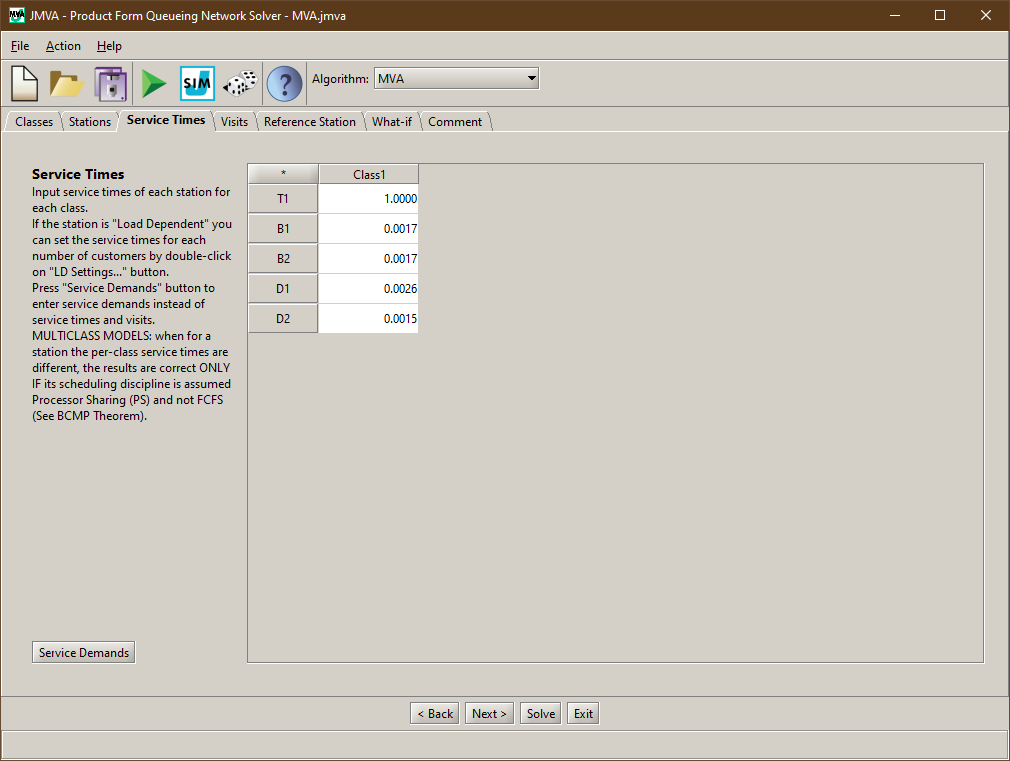
\includegraphics[scale=0.4]{004/JMVA/service_times.png}
	\caption{JMVA setup -- service times}
\end{figure}

4.
The relative visit ratios previously calculated for each station are entered.
\begin{figure}[h]
	\centering
	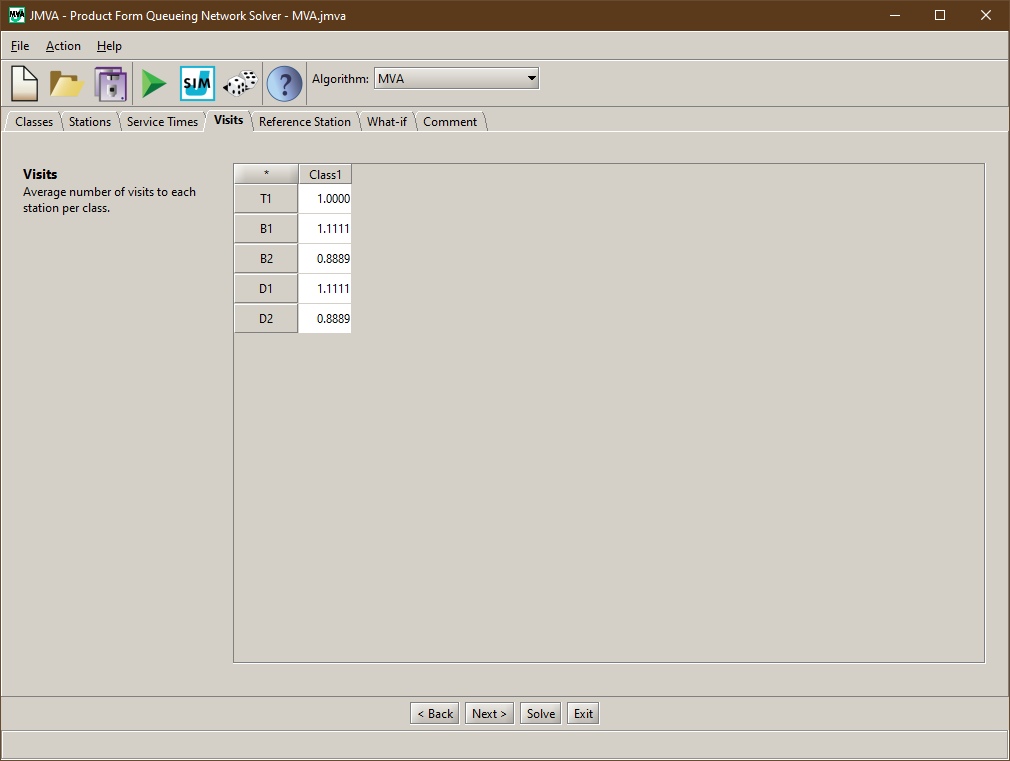
\includegraphics[scale=0.4]{004/JMVA/visits.png}
	\caption{JMVA setup -- relative visit ratios}
\end{figure}

\clearpage

5.
The reference station of the queueing network is indicated.
\begin{figure}[h]
	\centering
	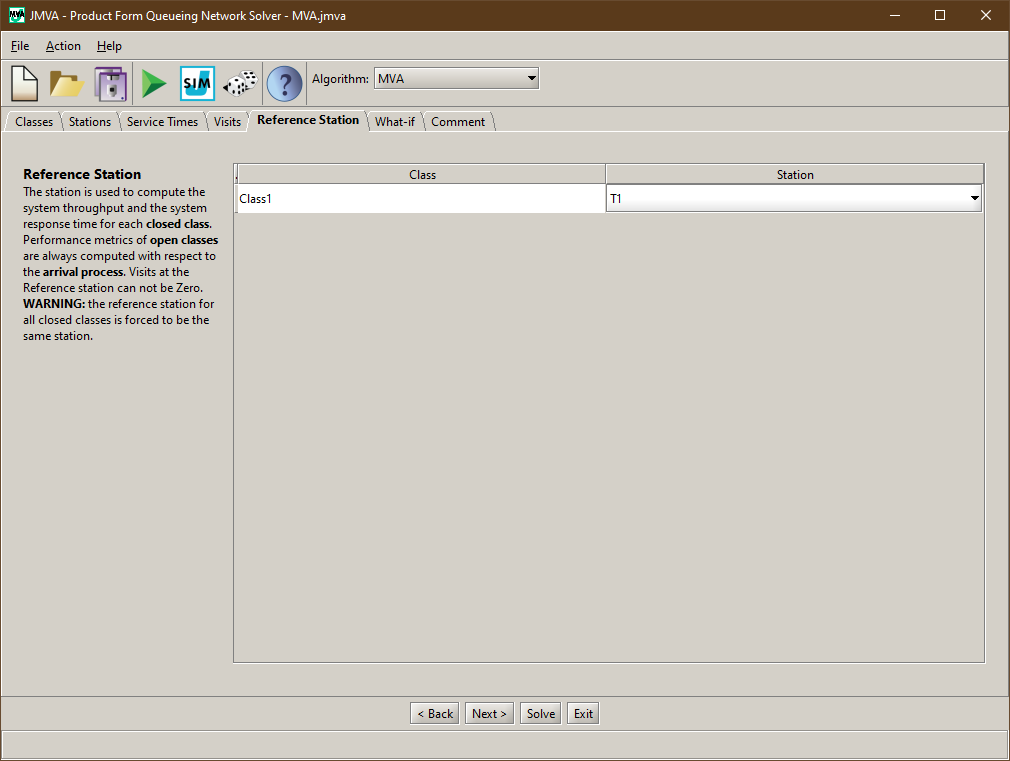
\includegraphics[scale=0.4]{004/JMVA/reference_station.png}
	\caption{JMVA setup -- reference station}
\end{figure}

6.
The initial number of users is indicated as 50, with a subsequent increment of up to 500 users per increment of 1 user.
\begin{figure}[h]
	\centering
	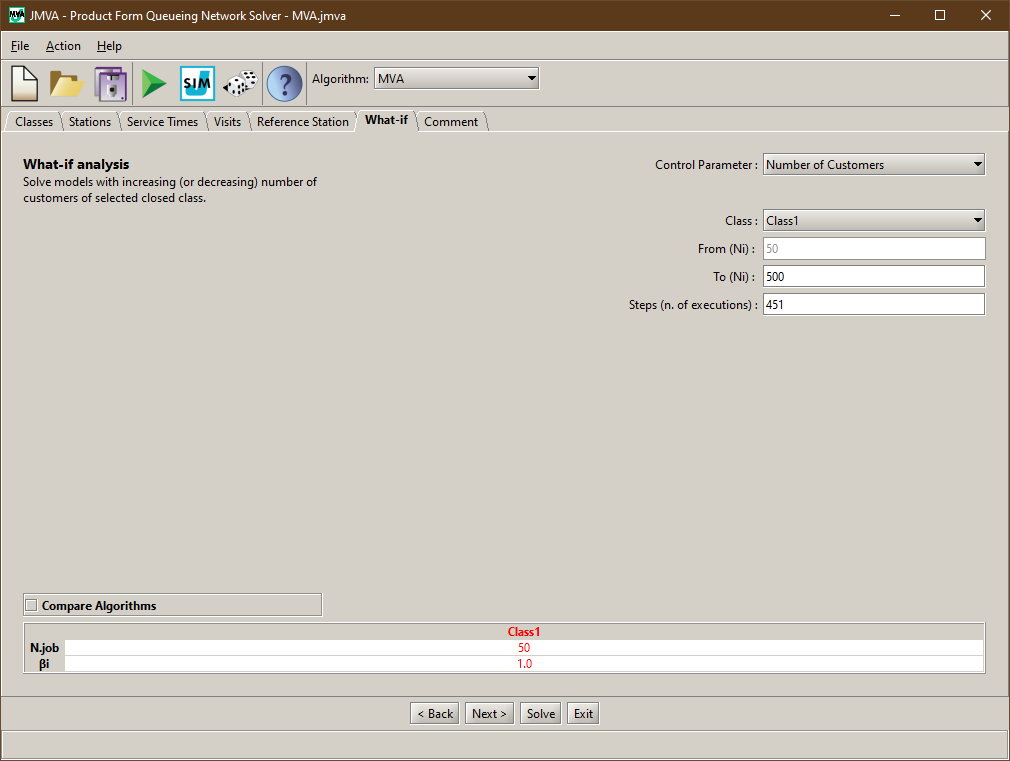
\includegraphics[scale=0.4]{004/JMVA/what_if.png}
	\caption{JMVA setup -- emulation settings}
\end{figure}

\subsection{JMVA emulation results}

The graphs generated by the emulation of JMVA, in conjunction with the previously calculated theoretical bounds, are presented below for the reader's convenience.
As can be observed in the graphs, the optimal number of users has already been determined; this will be calculated in the following section.

\begin{figure}[h]
	\centering
	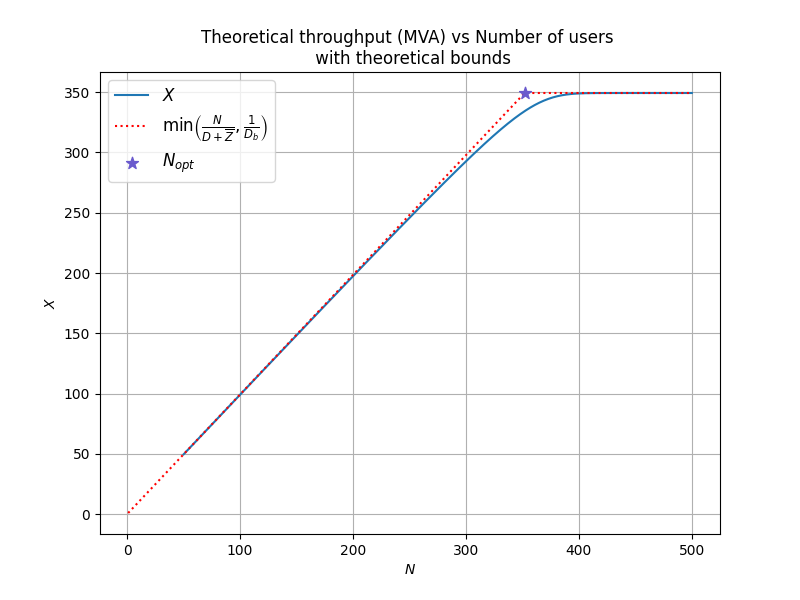
\includegraphics[width=\linewidth]{004/mva-x.png}
	\caption{MVA -- Throughput over the number of users}
\end{figure}

\begin{figure}[h]
	\centering
	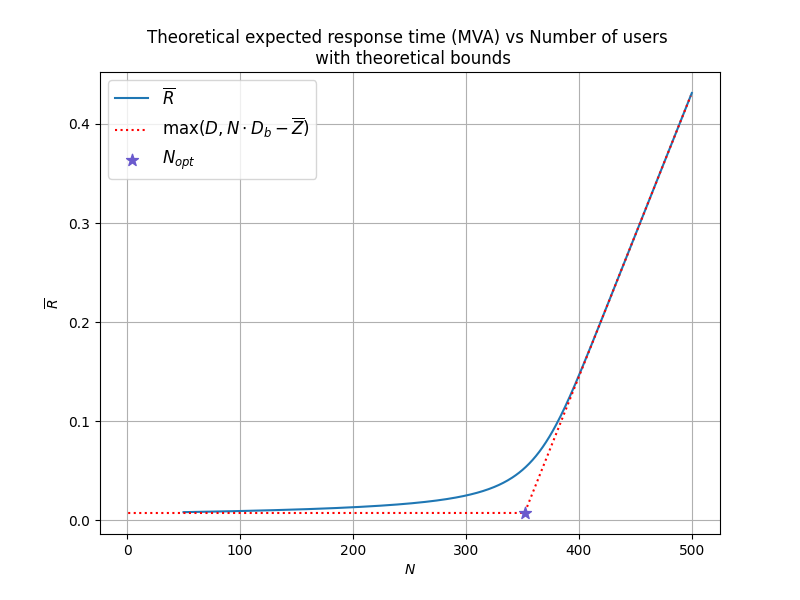
\includegraphics[width=\linewidth]{004/mva-r.png}
	\caption{MVA -- Response time over the number of users}
\end{figure}

\clearpage

\section{Optimal -- theoretical -- number of users}

In conclusion to the theoretical analysis of the queuing network, we proceed with the estimation of the optimal number of users.
This can be obtained from the intersection of the previously calculated asymptotes for throughput and expected response time and with the following formula:

\label{eq:optimal-number-of-users}
\begin{equation}
	N_{opt} = \frac{\overline{D} + \overline{Z}}{\overline{D}_b} = \num[round-mode=places, round-precision=5]{351.986511402232}
\end{equation}

The outcome is fully reflected in the graphs illustrated above.


\chapter{Q.N. Empirical analysis}
This chapter will address the core experimental aspect of the assignment: the configuration of the load test and the procedure by which it is launched.
Subsequently, the final experimental outcomes will be presented.

\section{JMeter – load test configuration}

In the ``User Defined Variables'' module, the address of the computer running the RESTful API was entered.
All other components of the load test are contained in a ``Transaction controller'', which allows the system's throughput and expected response time to be measured, rather than the user's.
\begin{figure}[h]
	\centering
	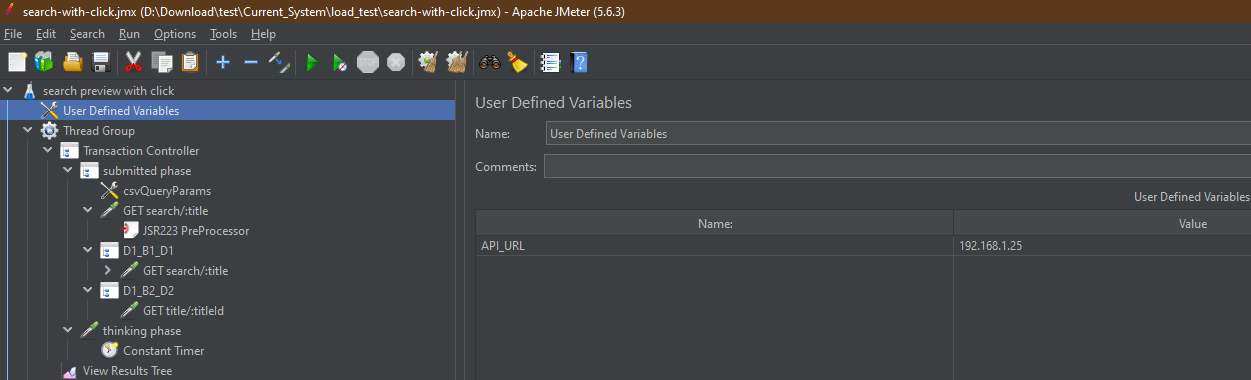
\includegraphics[width=\linewidth]{005/jmt-user-defined-variable.png}
	\caption{JMT -- User Defined Variables}
\end{figure}

\clearpage

In the ``Thread Group'' module, a population of 500 users was specified (this value will be updated automatically).
The \textit{ramp-up} period is 0, which means that when the test is initiated, all threads are simultaneously spawned in the thinking station.
The \textit{loop count} is infinite, which means that requests to the API will continue indefinitely, based on the query set imported via CSV.
The thread lifetime (\textit{duration}) is 10 minutes, after which it will eventually die.
\begin{figure}[h]
	\centering
	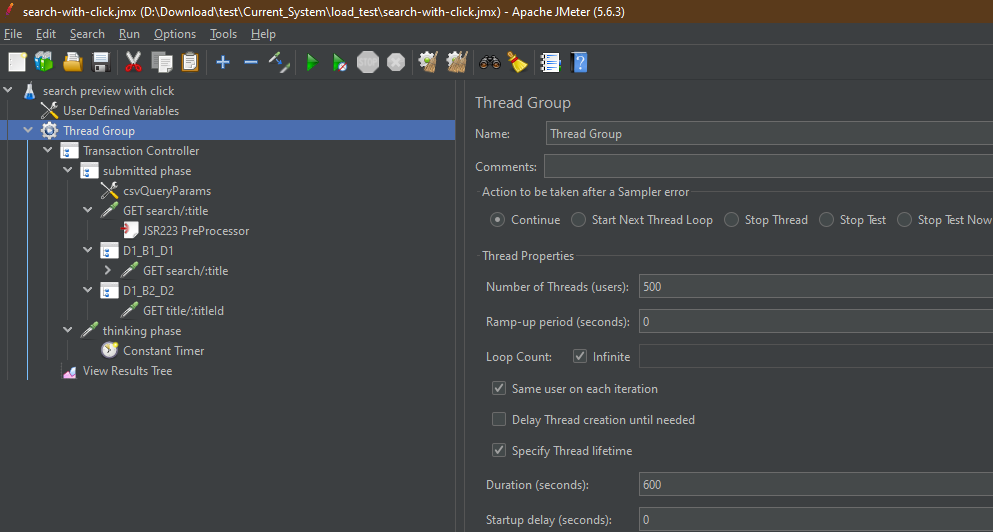
\includegraphics[width=\linewidth]{005/jmt-thread-group.png}
	\caption{JMT -- Thread Group}
\end{figure}

In the ``csvQueryParams'' module, the location of the CSV file containing the query set of 10,000 entries was specified.
The file will be read cyclically by each thread and will also be shared among them, which will therefore start reading it from different rows.
\begin{figure}[h]
	\centering
	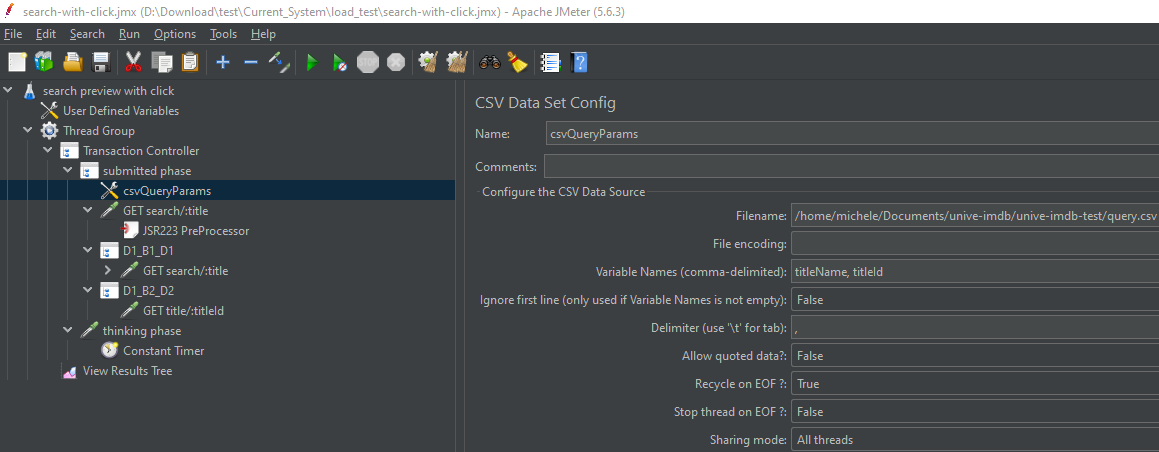
\includegraphics[width=\linewidth]{005/jmt-csv-query-params.png}
	\caption{JMT -- CSV Query Params}
\end{figure}

\clearpage

In this ``JSR223 PreProcessor'' module, the page number, which will subsequently be used to parameterize the API request ``\verb|/search/:title?page=n|'', is initialised to 1.
Additionally, a variable responsible for probabilistic routing, which will take values between 1 and 10 inclusive, is also initialised.
\begin{figure}[h]
	\centering
	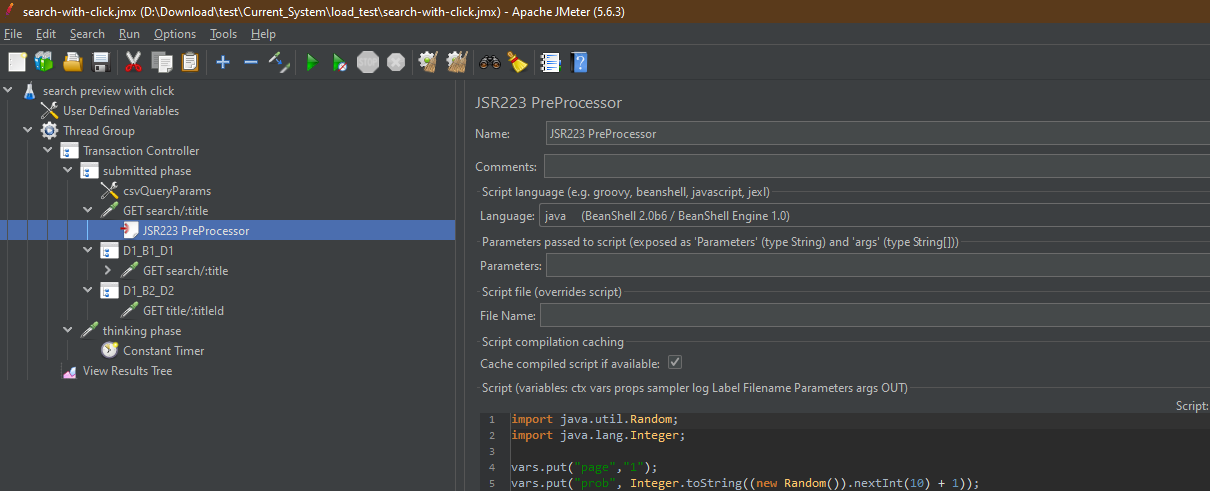
\includegraphics[width=\linewidth]{005/jmt-preproc-1.png}
	\caption{JMT -- JSR223 PreProcessor (1)}
\end{figure}

In this ``HTTP Request'' module, a request is submitted to the \newline ``\verb|/search/:title?page=1|'' endpoint.
\begin{figure}[h]
	\centering
	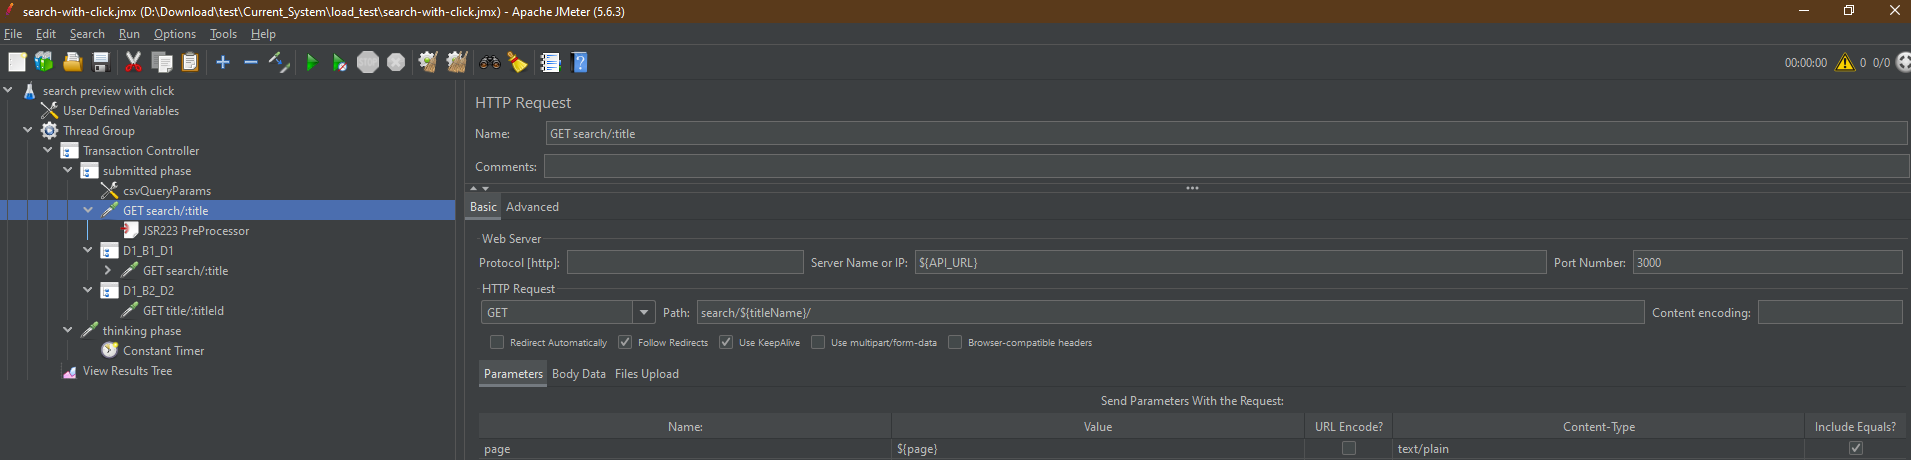
\includegraphics[width=\linewidth]{005/jmt-search-p1.png}
	\caption{JMT -- HTTP Request (1)}
\end{figure}

\clearpage

In the ``While Controller'' module, we test whether the user is within the 10\% probability of repeating the title search with an updated pagination value.
\begin{figure}[h]
	\centering
	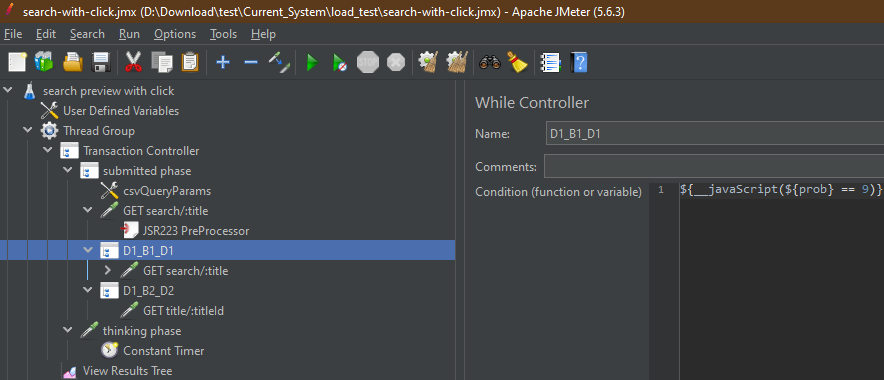
\includegraphics[width=\linewidth]{005/jmt-while.png}
	\caption{JMT -- While Controller}
\end{figure}

In this ``JSR223 PreProcessor'' module, the page number is incremented in accordance with the occurrence of the event in which the search is reiterated.
\begin{figure}[h]
	\centering
	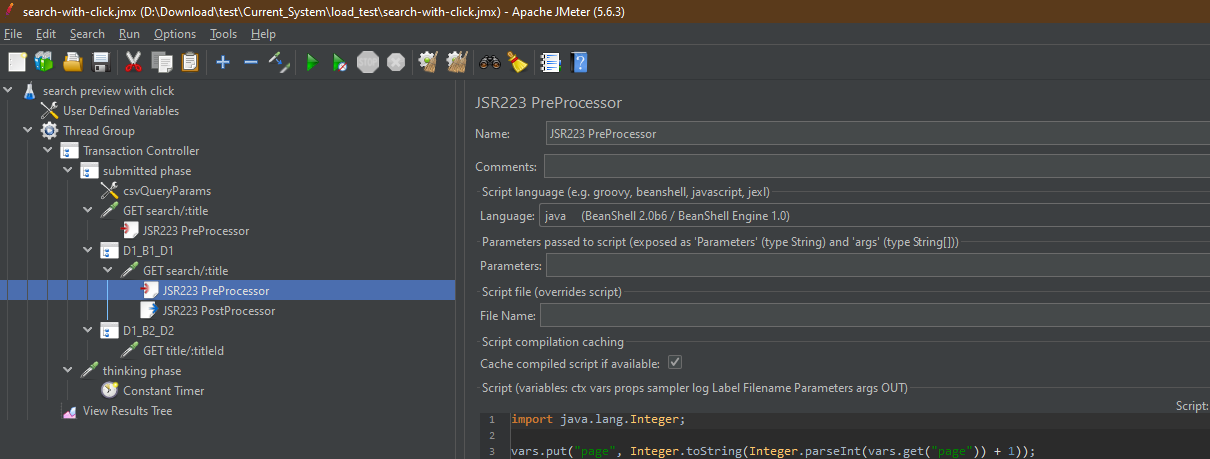
\includegraphics[width=\linewidth]{005/jmt-preproc-2.png}
	\caption{JMT -- JSR223 PreProcessor (2)}
\end{figure}

\clearpage

In this ``HTTP Request'' module, a request is submitted to the \newline ``\verb|/search/:title?page=n|'' endpoint.
\begin{figure}[h]
	\centering
	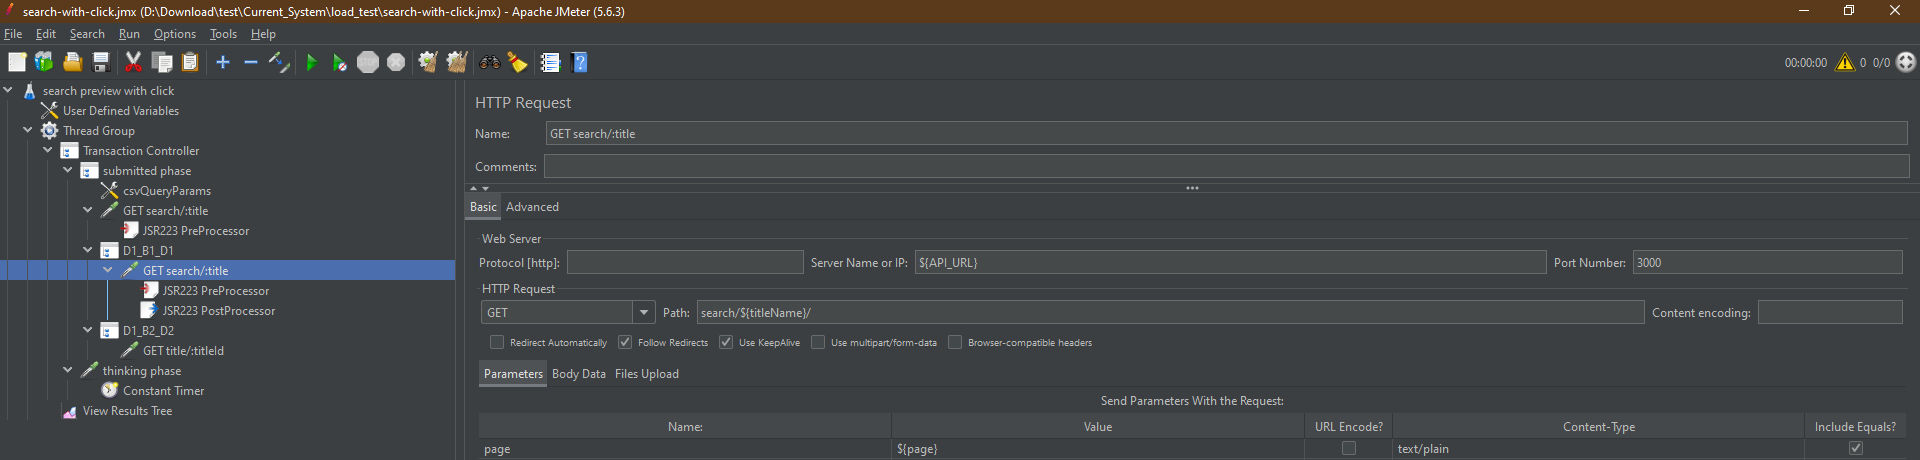
\includegraphics[width=\linewidth]{005/jmt-search-pn.png}
	\caption{JMT -- HTTP Request (2)}
\end{figure}

In the ``JSR223 PostProcessor'' module, the value is reassigned to the variable responsible for probabilistic routing.
\begin{figure}[h]
	\centering
	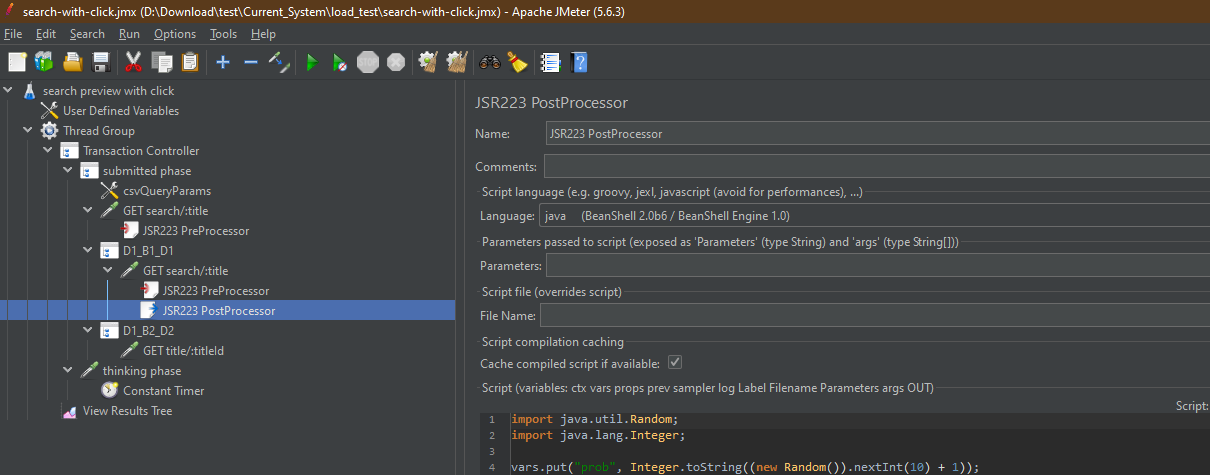
\includegraphics[width=\linewidth]{005/jmt-postproc.png}
	\caption{JMT -- JSR223 PostProcessor}
\end{figure}

\clearpage

In the ``If Controller'' module, we assess whether the user is within the 80\% probability of performing a precise search to retrieve the title or episode information.
\begin{figure}[h]
	\centering
	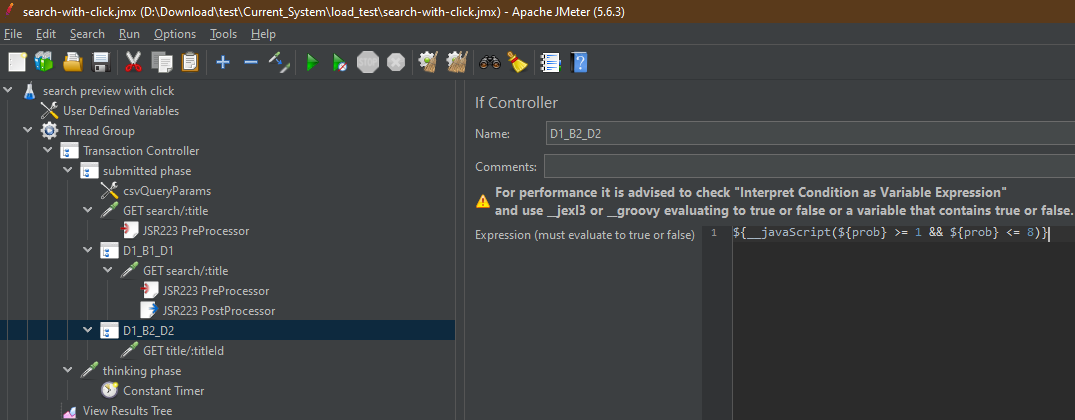
\includegraphics[width=\linewidth]{005/jmt-if.png}
	\caption{JMT -- If Controller}
\end{figure}

In this ``HTTP Request'' module, a request is submitted to the ``\verb|/title/:id| \textit{or} \verb|/episode/:id|'' endpoint.
\begin{figure}[h]
	\centering
	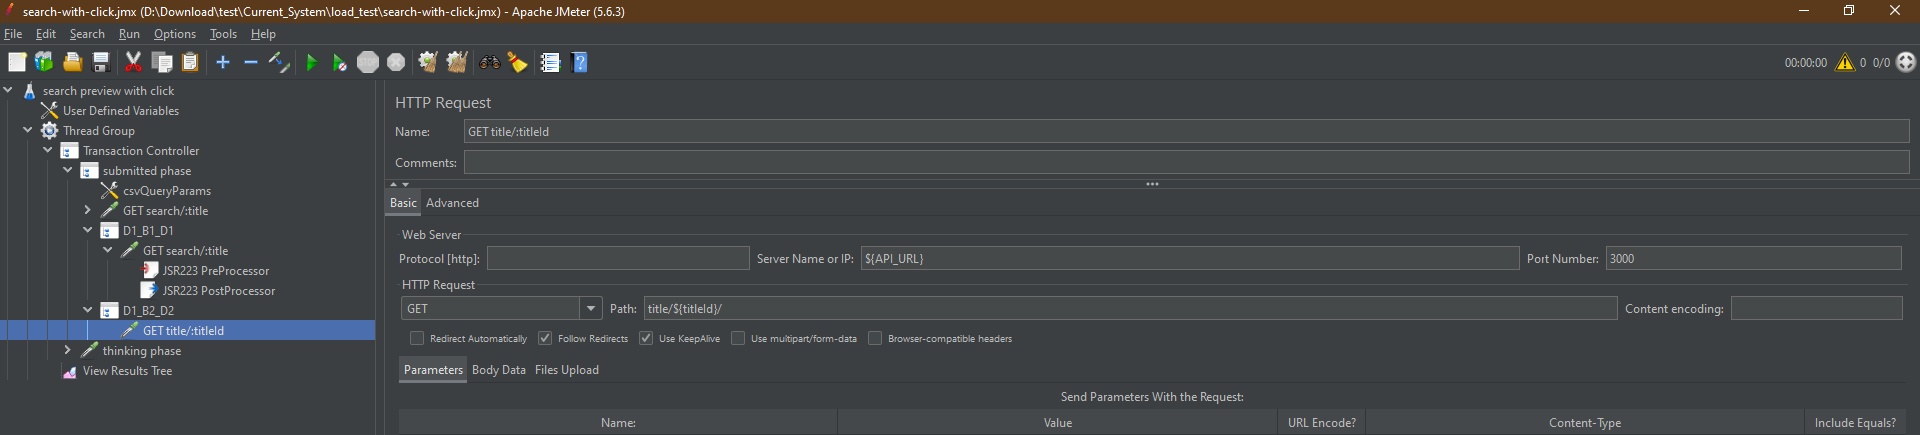
\includegraphics[width=\linewidth]{005/jmt-search-title.png}
	\caption{JMT -- HTTP Request (3)}
\end{figure}

\clearpage

In the ``Constant Timer'' module, the thinking time of 1 second is defined as the period of time that a thread will wait at the conclusion of one of its cycles before initiating a new one.
\begin{figure}[h]
	\centering
	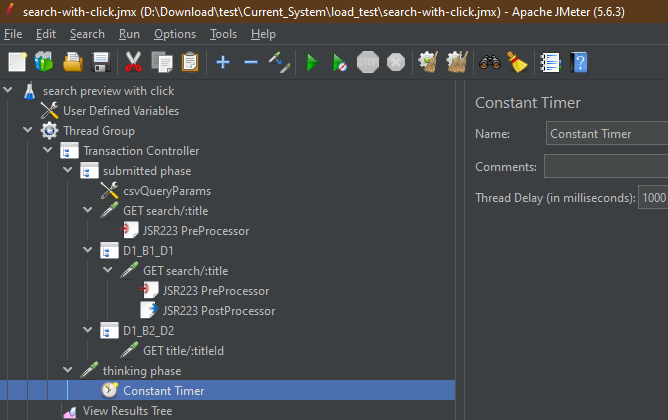
\includegraphics[width=\linewidth]{005/jmt-thinking-time.png}
	\caption{JMT -- Constant Timer}
\end{figure}

\section{Load test execution}

\subsection{Express and MongoDB configuration}

Prior to executing the load test, it is of crucial importance to ensure that the RESTful API and the database have been properly configured.

With regard to Express, it is necessary to compile and subsequently run the testing version of the script, which is relieved of profiling mechanisms and is also controlled by \verb|nodemon|\footnote[1]{https://nodemon.io/}, a Node.js npm package that among its various features automatically restarts the service when an error occurs.

With regard to MongoDB, it is essential to ensure that the Query Plan Cache is free of any residual data.
This can be achieved by executing the command \verb|db.collection.getP|\newline\verb|lanCache().clear()| within \verb|mongosh|.
Furthermore, it is necessary to disable the MongoDB Profiler by executing \verb|db.setProfilingLevel(0, { <options> })|.
Finally, if desired, the Profiler collection can be cleared with \verb|db.system.profile.drop()|.

It should be noted that the testing version of the RESTful API has been equipped with a mechanism to automatically clear the database cache after each query.
This is to prevent the distortion of test results due to caching mechanisms, which could otherwise occur if identical sequential queries were to be executed.

\subsection{Automated load test startup}

To ensure an absolute minimum of potential error in the load testing process, it was deemed appropriate to employ a Python utility for this specific purpose. 
The implemented source code is responsible for importing the load test configuration file, which was exported from JMeter in the jmx format, using the \verb|beautifulsoup|\footnote[2]{https://www.crummy.com/software/BeautifulSoup/} library.

Subsequently, the actual load test is initiated through the \verb|subprocess| library, which launches 10 sequential tests with a varying number of customers (threads), ranging from 50 to 500.

\vspace{8mm}

\begin{lstlisting}[language=Python, caption={Python script for automated load test startup}, label={lst:python-script}]
import subprocess
from tqdm import tqdm
from bs4 import BeautifulSoup

def test(name:str):
 jmx_name=f'{name}.jmx'

for n_users in tqdm(range(50, 550, 50)):      
 with open(jmx_name) as f:
  Bs_data = BeautifulSoup(f.read(), "xml")
  tag=Bs_data.find('intProp', {"name":"ThreadGroup.num_threads"})
  tag.string = str(n_users)

with open(jmx_name, 'w') as f:
 f.write(str(Bs_data))
 results_path = f'results_{n_users}'
 subprocess.Popen(f'jmeter -n -t {jmx_name} -l {results_path+"/results.csv"} -e -o {results_path}', shell=True, stdout=subprocess.DEVNULL).wait()

if __name__ == "__main__":
 test('filename')
\end{lstlisting}

\section{Experimental results}

The graphs of throughput and expected response time, calculated from the load test performed with JMeter, are presented below.
The graphs were generated following a parsing step of the statistics exported in JSON format from the benchmark software.

\clearpage

\begin{figure}[h]
	\centering
	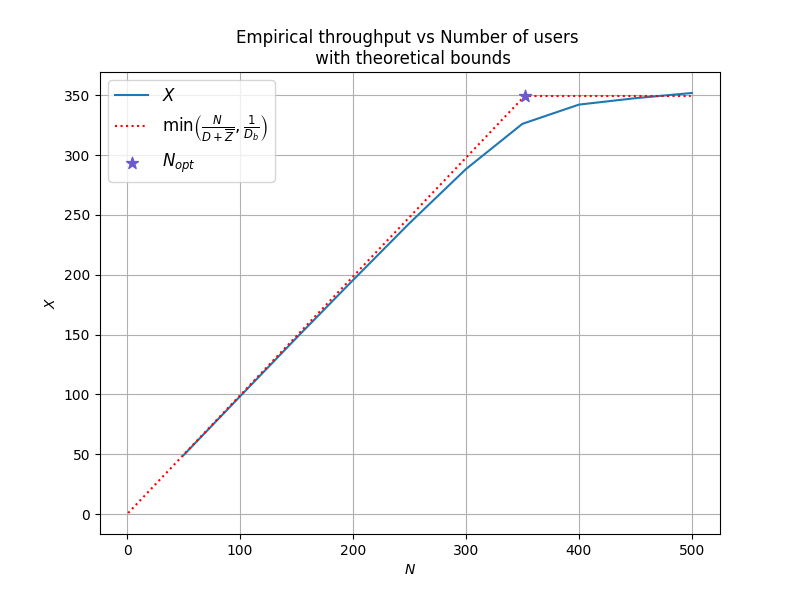
\includegraphics[width=\linewidth]{005/load-test-x.png}
	\caption{JMeter Load test -- Throughput}
\end{figure}

\clearpage

\begin{figure}[h]
	\centering
	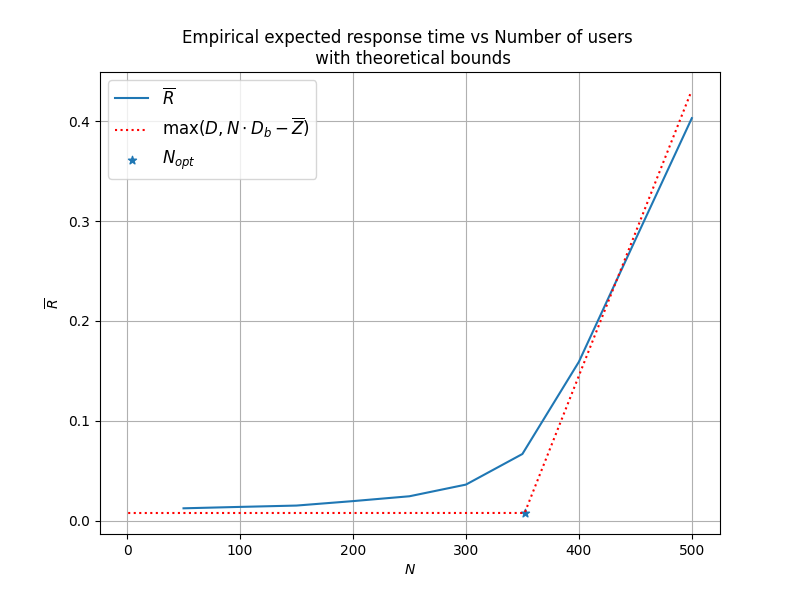
\includegraphics[width=\linewidth]{005/load-test-r.png}
	\caption{JMeter Load test -- Expected Response Time}
\end{figure}

The graphs demonstrate a satisfactory fit with respect to the analytically calculated asymptotes.
Additionally, they illustrate the precision of the estimated optimal number of users that the system can handle, which was previously determined through analysis.


\begin{comment}
Capitolo 6: Conclusioni
	- Proposta di architettura scalabile.
		- MongoDB caching.
		- MongoDB Sharding e replica.
		- Implementazione (nuovo disegno, e traffic equations) ...dispatcher ?
		- Analisi prestazioni sistema proposto con MVA.
\end{comment}

\end{document}
